\documentclass{article}

% New commands declaration

\usepackage[frenchb]{babel}
\usepackage[T1]{fontenc}

\usepackage{natbib,bibentry}
\usepackage{color}
\usepackage{listings}

\usepackage{yfonts}
\usepackage{graphicx}
\usepackage{epsfig,subfigure}
\usepackage{amsmath,amssymb,amsfonts}
\usepackage{calc}
\usepackage{import}

\DeclareGraphicsExtensions{.eps, .jpg, .png}
\DeclareMathOperator*{\argmin}{argmin}

\parindent = 0mm

\bibliographystyle{plain}

\hoffset = -20mm
\voffset = -25mm
\textwidth = 160mm
\textheight = 240mm

\definecolor{lightgray}{gray}{0.2}
\definecolor{mygreen}{RGB}{28,172,0}
\definecolor{mylilas}{RGB}{170,55,241}

\newcommand{\expect}{{\rm I \mkern-2.5mu \nonscript\mkern-.5mu E}}
\newcommand{\equaldef}{\stackrel{d}{=}}
\newcommand{\argmax}{\operatornamewithlimits{argmax}}

\newcommand{\debutrep}[1]{\color{blue}\begin{center} \hrulefill \textbf{ #1 } \hrulefill \end{center} }
\newcommand{\finrep}{\vspace*{5mm}\hfill $\square$\color{black}\vspace*{5mm}}

\begin{document}

\lstset{language=Matlab,%
    %basicstyle=\color{red},
    breaklines=true,%
    morekeywords={matlab2tikz},
    keywordstyle=\color{blue},%
    morekeywords=[2]{1}, keywordstyle=[2]{\color{black}},
    identifierstyle=\color{black},%
    stringstyle=\color{mylilas},
    commentstyle=\color{mygreen},%
    showstringspaces=false,%without this there will be a symbol in the places where there is a space
    numbers=left,%
    numberstyle={\tiny \color{black}},% size of the numbers
    numbersep=9pt, % this defines how far the numbers are from the text
    emph=[1]{for,end,break},emphstyle=[1]\color{red}, %some words to emphasise
    %emph=[2]{word1,word2}, emphstyle=[2]{style},    
}

\baselineskip = 4mm
\title{Optimisation et problèmes inverses: \\
TP1 - Descente de gradient}

\author{\textbf{4 ETI -- CPE Lyon }\\[3mm]
{Travaux Pratiques Optimisation}}
\date{2020-2021}

\maketitle

\noindent\fbox{
\parbox{\linewidth-2\fboxrule-2\fboxsep}
{ 
\vspace*{2mm}
{\large\bf Noms, Prénoms: Dorian FABREGUE, Axel BRUYERE }\\[3mm]
{\large\bf Spécialité: IMI }\\[3mm]
{\large\bf Date: 07/03/2021}\\[2mm]}}
\vspace*{5mm}



{\Large\bf Objectifs}~--~~\begin{minipage}[t]{135mm}
• Compréhension de l’algorithme de descente de gradient\\
• Compréhension de l’apport de la méthode numérique par rapport à une résolution directe\\
• Compréhension des limites de l’algorithme\\
• Compréhension du modèle des moindres carrés\\
• Compréhension du modèle de Tikhonov\\
• Compréhension des limites des modèles\\
• Implémentation de l’algorithme pour la minimisation des modèles des moindres carrés et de
Tikhonov en 1D et en 2D\\
\end{minipage}

\vspace*{4mm}
\renewcommand{\thesection}{\Roman{section}}

\section{Contexte}

On se concentrera dans ce TP sur des exemples en débruitage et déconvolution 1D (signal) et 2D
(image). Pour autant, nous rappelons que l’optimisation est un domaine transversal, et permet, en
fonction du choix de la fonction de coût, de traiter de nombreuses applications.\\
En particulier, on veut dans ce TP déruiter l’image ci-dessous :
\begin{figure}[h]
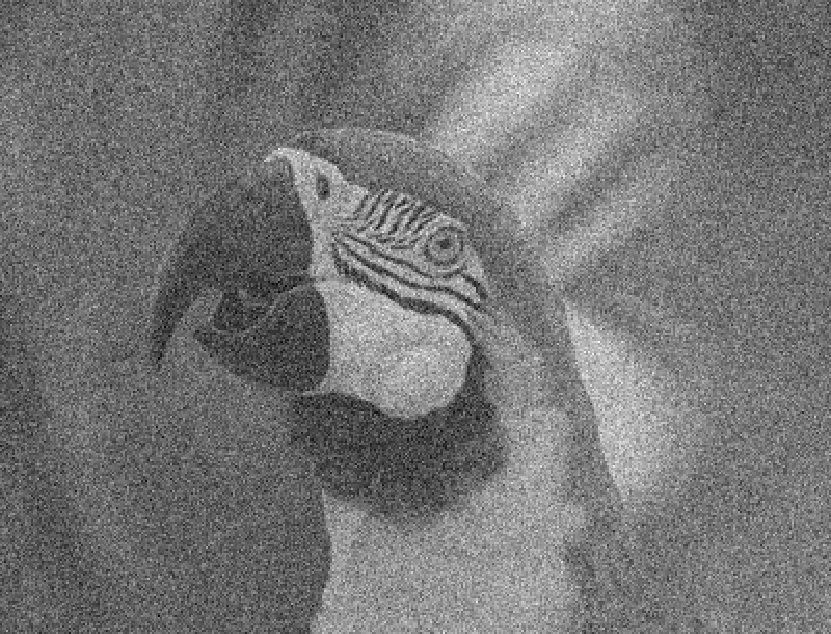
\includegraphics[width=8cm]{perroquet_original.png}
\centering
\end{figure}

\clearpage

\section{Prise en main de la méthode}

Pour étudier le principe de la méthode de gradient, on se propose d’appliquer l’algorithme pour
minimiser la fonction $f(x) = x^2 $, i.e. résoudre le problème de minimisation 1D:\\
\begin{equation}
\hat{x} = \argmin_{x \in \mathbb{R^N}}||x||_2^2
\label{eq:AR(M)}
\end{equation}
Nous allons pour cela mettre en place un algorithme de descente de gradient. 
\subsection{Algorithme de descente de gradient}
Le but d'un algorithme de descente est de construire une suite $(x_n)_n$ qui converge vers la valeure $\hat{x}$ souhaitée. Dans le cas de la descente de gradient, et grâce aux formules de développement de Taylor, chaque itération est dee la forme: $x_{k+1} = x_k - t_k \nabla f(x_k)$   avec $t_k$ le pas de descente.\\\\
Cependant la descente de gradient doit vérifier plusieurs critères afin de garantir la convergence de la suite $(x_k)_k$ vers  $\hat{x}$:\\
- $f:\mathbb{R^N} \rightarrow ]-\infty,+\infty]$ convexe, propre et semi-continue inférieurement, de gradient $\nu$-Lipschitz, $\nu\in]0,+\infty[$, tq $\argmin f \neq \emptyset$ \\
- $t_k$ une suite dans $[\underline{\rm t},\overline{\rm t}]$ tq $0\leq\underline{\rm t} \leq \overline{\rm t} \leq \frac{2}{\nu}$ \\
- $x_0 \in \mathbb{R^N}$. \\
On sait que la fonction norme $f:x \rightarrow ||x||_2^2$ vérifie facilement ces critères. Il nous reste à déterminer un pas $t_k$ et de choisir un $x_0 \in \mathbb{R^N}$.

\subsection{Mise en pratique}
Nous codons cette suite $(x_k)_k$ sous Matlab, sachant que celle-ci doit normalement converger vers $\hat{x}  = \argmin_{x \in \mathbb{R^N}}||x||_2^2 = 0$. Les valeurs de la dimension de X, du pas d'itération et de la précision éxigée sont ici choisies de manière arbitraire.
\\
{
\color{blue}
\begin{verbatim}
df = @(x) 2*norm(x);
N=5;
X=randn([N 1]);

%Suite x_k
k = 0; pas = 0.4; aim = 1.0e-06; max_it = 10000;

while (abs(df(X))>aim && k<max_it)
    X= X - 2*pas*X;
    k = k + 1;
end

\end{verbatim}
}

Nous avons obtenu les résultats suivants:\\
$X = [1.06\times10^{-7}; 7.44\times10^{-08}; -3.10\times10-08; 3.00\times10^{-08}; -8.06\times10^{-08}] \approx  \hat{x} $\\
$k=10$ (compteur)\\ \\
Un problème de cet algorithme réside dans un choix correct du pas de descente: si celui-ci est trop faible, le nombre d'itérations nécessaires sera trop important, et à l'nverse, si celui-ci est trop grand nous sortons des critères de convergence définis précédemment.\\

\begin{figure}[h]
\centering

\caption{figure}
\end{figure}


\vspace*{3mm}

\subsection{Choix du pas de descente optimal}
Précédemment, nous avons défini un pas de descente constant $\forall k, t_k = 0,4$. Nous allons chercher ici à déterminer une règle de calcul d'un $t_k$ optimal proche de $\frac{2}{\nu}$.\\
En premieur lieu, on peut penser à réaliser une recherche linéaire du $t_k$ à chaque itération jusqu'à obtenir sa valeur optimale. On sait que la recherche linéaire est une méthode couteuse, surtout quand cell-ci est répétée à chaque itération.  \\\\
Afin de réduire ce coût, nous utiliserons la règle d'Armijo: $\forall k$, on choisit $t_k$ et on teste si $f(x_k - t_k\nabla f(x_k)) < f(x_k)$, tant que ce n'est pas le cas, on choisit $t_k\frac{t_k}{c}$
\clearpage

\section{Introduction aux différentes fonctions de coût }
Nous avons vu en cours que les fonctions de coût en image sont de la forme
\begin{equation}
f(x) = L(Hx;z) + \lambda R(x)
\end{equation}

où L est l’attache aux données (choisie en fonction du type de dégradation) et R est une régularisation
(choisie en fonction du type de résultat souhaité).\\
Nous allons ici étudier l'influence de chaque termes.

\subsection{Modèle des moindres carrés}
On se concentre dans un premier temps sur une fonction de coût sans régularisation (i.e. $f (x) = L(Hx;z)$). Dans le cas d’une dégradation par un flou $H$ etun bruit gaussien, le problème de minimisation est donc réduit au modèle des moindres carrés, défini par :
\begin{equation}
\hat{x} = \argmin_{x \in \mathbb{R^N}}||Hx-z||_2^2
\label{eq:AR(M)}
\end{equation}
On pourra se limiter dans un premier temps au choix $H = Id$. Une fois la méthode implémentée, on pourra introduire une dégradation $H$ de type flou et/ou décimation.

\subsection{Modèle de Tikhonov 1D}
On souhaite étudier l’influence de la régularisation R. L’un des modèles les plus connus (utilisé par
exemple pour la reconstruction tomographique) en traitement d’image est le modèle de Tikhonov,
défini de la manière suivante :
\begin{equation}
f(x) = L(Hx;z) + \lambda||\Gamma x||^2_2
\end{equation}
où $\Gamma$ modélise un opérateur de notre choix (identité, gradient, Laplacien...).


\subsection{Modèle de Tikhonov 2D}
\debutrep{code}
\begin{verbatim}

\end{verbatim}
\finrep

\debutrep{résultats}
\begin{figure}[h]
\centering

\caption{figure}
\end{figure}
\finrep

\vspace*{3mm}

\subsection{Analyse des résultats}

\clearpage


\section{Résolution du modèle de Tikhonov 1D}
Insérer texte

\subsection{Programmation et résultats}
Insérer texte
\debutrep{code}
\begin{verbatim}

\end{verbatim}
\finrep

\debutrep{résultats}
\begin{figure}[h]
\centering

\caption{figure}
\end{figure}
\finrep


\subsection{Analyse des résultats}

\clearpage


\section{Résolution du modèle de Tikhonov 2D}
Insérer texte

\subsection{Programmation et résultats}
Insérer texte
\debutrep{code}
\begin{verbatim}

\end{verbatim}
\finrep

\debutrep{résultats}
\begin{figure}[h]
\centering

\caption{figure}
\end{figure}
\finrep

\vspace*{3mm}

\subsection{Analyse des résultats}

\clearpage





\end{document}

